\chapter{Results}

This section summarizes the results that the described algorithm achieved on the described datasets according to the described metrics. Before going into detail about the performance on the Siddata-dataset, a brief summary of the results on the placetypes-dataset serves to demonstrate if the specific implementation can achieve comparable results to \mainalgos, thus putting the other results into perspective in terms of what the algorithm can realistically achieve on dedicated high-quality datasets.

% Due to the implemented algorithm being an \gls{unsupervised} algorithm, there is no explicit target value for each of the considered samples, making it impossible to straight-forwardly apply well-known \gls{ml} metrics such as \Gls{acc} or \gls{f1}. What this algorithm tries to achieve is a lot \textit{fuzzier} than in the realm of classification: The end-goal of it is to embed the given \glspl{entity} into a vector-space that consists of semantically meaniningful directions, so the only actual metric would be a comparison checking if the respective categorization here corresponds closely to human judgement. To do that, the best evaluation is likely a study that asks for feedback of users that see the results of a developed system\footnote{An example for such a system is the \textit{Movie Tuner} interface from \textcite{VISR12}, reprinted as \autoref{fig:movetuner}.}. \textcite{Derrac2015} performed crowdsourcing experiments on CrowdFlower\footnote{\url{http://www.crowdflower.com}}, asking users among other tasks which of several candidates could best describe the difference between two movies. They also compared their results with those of running the supervised algorithm of \cite{VISR12} on a subset of their data. Furthermore they tested if the explainable classifiers generated from this algorithm (see \autoref{sec:reasoning}) \q{help users spot incorrect classifications} \cite[48]{Derrac2015}, as well as if their algorithmic classification corresponds to human judgement\footnote{The task was set only for classification into OpenCYC and Foursquare Taxonomies of the placetypes-dataset (see column `\textbf{classification classes}' in \autoref{tab:all_datasets}).}. 
% \todoparagraph{TODO: Should I also quickly mention their results?}
% While similar studies could be done in the Siddata-\gls{dsa} \cite{Schurz2021} without additional costs, carrying these out is outside the scope of this thesis.


% This thesis relies on both qualitative analysis and quantitative anlaysis in order to quantify the algorithm's performance. In the \textit{qualitative analysis}, exemplary partial results of the algorithm will be showcased that should intuitively show if what the algorithm does looks \textit{realistic} from a human perspective. 

\section{Replicating the results for placetypes}
\label{sec:results_placetypes}

To check if the implementation correctly produces the claimed results, it was applied to \gencite{Derrac2015} placetypes-dataset and its results compared to those of the literature. \autoref{fig:scatter_mds_placetypes} in \autoref{ap:more_plots} shows a two-dimensional \gls{tsne}-embedding of the original representations of \cite{Derrac2015}, colored by their Geonames-class. This figure indicates that only few of the entities are linked with a class and that the embeddings barely cluster when compared to their embeddings for the movies-dataset (displayed in \autoref{fig:scatter_mds_movies}). 

Both \cite{Ager2018} and \cite{Alshaikh2020} report the performance of depth-1, depth-3 and unbounded decision trees classifying an entities' category according to the Placetypes- and Geonames-taxonomy. \autoref{tab:f1_mainalgos_me_short} lists their results as well as some of their baselines in comparison with the results of this work. As shown in the table, this implementation outperforms the previous results for all configurations. \autoref{tab:f1_geonames_foursquare_all} shows the results of different configurations to generate the decision-tree classification. In contrast to the results reported in \ref{tab:f1_mainalgos_me_short} which are optimized for their respective classification target, these results are from a single parameter-combination and robustly reproducible. 

\begin{table}[H]
	\begin{subtable}{.627\linewidth}
		\centering
		\resizebox{\textwidth}{!}{
			\begin{tabular}{rrcccc}
				\toprule
				 & \textbf{Depth} & \textbf{-} & \textbf{1} & \textbf{2} & \textbf{3} \\
				\textbf{1vsRest} & \textbf{Balanced} &  &  &  &  \\
				\midrule
				\multirow[t]{2}{*}{\textbf{False}} & \textbf{False} & 0.377 & {\cellcolor{lightgreen}} 0.484 & {\cellcolor{lightgreen}} 0.496 & 0.496 \\
				 & \textbf{True} & 0.394 & 0.134 & 0.238 & 0.256 \\
				\cline{1-2}
				\multirow[t]{2}{*}{\textbf{True}} & \textbf{False} & 0.424 & 0.320 & 0.332 & 0.366 \\
				 & \textbf{True} & {\cellcolor{lightgreen}} 0.441 & 0.482 & 0.489 & {\cellcolor{lightgreen}} 0.513 \\
				\bottomrule
			\end{tabular}
		}
		\caption{GeoNames}\label{tab:f1_geonames_all}
	\end{subtable}%
	\begin{subtable}{.373\linewidth}
		\centering
		\resizebox{\textwidth}{!}{
			\begin{tabular}{cccc}
				\toprule
				\textbf{-} & \textbf{1} & \textbf{2} & \textbf{3} \\
				&  &  &  \\
				\midrule
				0.506 & 0.330 & 0.417 & 0.455 \\
				{\cellcolor{lightgreen}} 0.550 & 0.113 & 0.294 & {\cellcolor{lightgreen}} 0.499 \\
				0.511 & 0.319 & 0.403 & 0.417 \\
				0.505 & {\cellcolor{lightgreen}} 0.451 & {\cellcolor{lightgreen}} 0.521 & 0.498 \\
				\bottomrule
			\end{tabular}
		}
		\caption{Foursquare}\label{tab:f1_foursquare_all}
	\end{subtable}
	\slcaption{F1-Scores of various-depth decision trees predicting GeoNames- and Foursquare-labels. All scores are the result of 5-fold cross-validation averaged across 10 random seeds, but from a single parameter-configuration. Rows correspond to different hyperparameters for the \gls{dt}. If not \textit{1vsRest}, a single tree must predict all classes at once (max. 2\textsuperscript{depth}).}.
	\label{tab:f1_geonames_foursquare_all}
\end{table}



\begin{table}[H]
	\centering
	% \resizebox{\textwidth}{!}{%
	\begin{tabular}{rr|ccc|ccc|cc}
	\textbf{Target} &
	  \textbf{Cls} &
	  \textbf{Ran} &
	  \textbf{LDA} &
	  \textbf{BL} &
	  \textbf{\cite{Derrac2015}} &
	  \textbf{\cite{Ager2018}} &
	  \textbf{\cite{Alshaikh2020}} &
	  \textbf{this work} \\ \midrule
	\textbf{Foursquare}  & \textbf{D1}  & 0.39 & \textbf{0.55} & -             & 0.38*          & 0.41 & \textbf{0.45} & \textbf{0.50} \\
						 & \textbf{D3}  & 0.5  & 0.48          & -             & 0.42*          & 0.44 & \textbf{0.57} & \textbf{0.58} \\
						 & \textbf{DN}  & -    & 0.47          & \textbf{0.53} & \textbf{0.53}  & 0.42 & -             & \textbf{0.57} \\
	\multicolumn{1}{l}{} & \textbf{Any} & -    & -             & 0.72          & \textbf{0.73}  & -    & -             & -             \\
	\textbf{Geonames}    & \textbf{D1}  & 0.23 & \textbf{0.34} & -             & \textbf{0.32*} & 0.32 & 0.28          & \textbf{0.51} \\
						 & \textbf{D3}  & 0.27 & 0.32          & -             & 0.31*          & 0.31 & \textbf{0.34} & \textbf{0.54} \\
						 & \textbf{DN}  & -    & 0.27          & 0.2           & \textbf{0.37}  & 0.24 & -             & \textbf{0.46} \\
	\multicolumn{1}{l}{} & \textbf{Any} & -    & -             & 0.36          & \textbf{0.41}  & -    & -             & -            
	\end{tabular}%
	% } %resizebox
	\slcaption{F1-Scores of classifiers predicting GeoNames- and Foursquare-labels for three baselines, \mainalgos and this work. \textbf{Cls} column encodes the classifier: \textbf{D1/3} are \glspl{dt} of depth 1/3, \textbf{DN} an unbounded \gls{dt}. Condition \textbf{Any} refers to the best of \cite{Derrac2015}'s  semantic classifiers. \hspace{1ex}
	Baseline-columns: \textbf{Ran} is the \textit{Random} baseline as reported by \cite{Alshaikh2020}, \textbf{LDA} is the result of \acrshort{lda} as reported by \cite{Ager2018}, and \textbf{BL} is the best baseline-condition from \cite{Derrac2015}. \hspace{1ex}
	Columns \textbf{\cite{Derrac2015}, \cite{Ager2018}} and \textbf{\cite{Alshaikh2020}} encode the best respectively reported scores. Starred values in column \textbf{\cite{Derrac2015}} refer to results that \cite{Ager2018} reported for the configuration of \cite{Derrac2015} for conditions not covered by the latter. Final column reports the results of this work (unlike \autoref{tab:f1_geonames_foursquare_all}, this reports the respectively optimal parameter-configuration) with a literature-consistent train-test-split of 70-30. A longer version of this table listing more configurations per author can be found in the Appendix as \autoref{tab:f1_placetypes_long}.}
	\label{tab:f1_mainalgos_me_short}
\end{table}


% \begin{table}[H]
% 	\resizebox{0.6\textwidth}{!}{%
% 	\caption{Results of the decision trees trained on }
% 	\label{tab:places_results}
% 	% möchte sagen: Wenn ich meine Sachen auf placetypes werfe hab ich comparable metrics -> my implementation is ok
% 	\begin{tabular}{llrrr}
% 	\toprule
% 	 & \textbf{Depth:} & \textbf{1} & \textbf{2} & \textbf{3} \\
% 	\textbf{1vsRest} & \textbf{Balanced} &  &  &  \\
% 	\midrule
% 	\multirow[t]{2}{*}{\textbf{False}} & \textbf{False} & 0.427 & 0.474 & 0.477 \\
% 	 & \textbf{True} & 0.057 & 0.107 & 0.139 \\
% 	\cline{1-2}
% 	\multirow[t]{2}{*}{\textbf{True}} & \textbf{False} & {\cellcolor{lightgreen}} 0.745 & {\cellcolor{lightgreen}} 0.795 & {\cellcolor{lightgreen}} 0.811 \\
% 	 & \textbf{True} & 0.529 & 0.660 & 0.681 \\
% 	\bottomrule
% 	\end{tabular}
% 	}
% \end{table}

\todoparagraph{Because of the big difference, we also report our results per param-combi and show that PPMI suuucks}


\section{Dataset differences} % Dataset comparisons (is our dataset worse?)
\label{sec:results_datasetdiffs}


Having established that the implementation works correctly for the domain of placetypes, we will now check if the quantity of some key characteristics produced as interim results of the algorithm differ across domains. \autoref{tab:generated_stuff} contrasts the number of feature vectors, candidate terms and cluster elements for the movies-, placetypes- and Siddata-dataset.

\todoparagraph{With that, we want to figure out if anything is possible and if so, the correct parameters like the candidate-min-term-count}

\begingroup
\begin{table}[H]
	\resizebox{\textwidth}{!}{%
		\centering
		\begin{tabular}{r|ccc|cc}
		& \multicolumn{3}{c}{\textbf{Feature vectors}}           & \textbf{Candidates} & \textbf{Cluster Elements}   \\
		& \textbf{Mean L.} & \textbf{Vectors} & \textbf{Clusters} &                     & \textbf{($\kappa\geq0.1$}) \\
		\midrule
		\textbf{movies \cite{Derrac2015}}     & 12\,083 & 589\,727 & 3\,864 & 22\,903 & 9\,389 \\
		\textbf{placetypes \cite{Derrac2015}} &         &          &        & 21\,833 &        \\
		\textbf{Siddata}                      &         &          &        & 10\,060 &        
		\end{tabular}
		\caption{Statistics on generated features of the algorithm}
		\label{tab:generated_stuff}
	}
\end{table}
\endgroup
% movies:
% feature vecs: 38649 keys with 0-33k terms each (sum: 589727 terms) 
% candidate-terms: 22903 (unclustered)
% clusters: ndims*2 -> for 20D: 9389 (-> 9429 words in $T^{0.1}$)}		
% movies: 15.000
% ppmi-weighted feature vectors: 38649 keys with bag-of-words between 0 words and 33k words (but mostly couple 1000s), all in all 589727 unique terms
% candidate-terms: 22903 (unclustered)
% clusters: ndims*2 clusters with all in all (for 20d) 9389 values (->9429 words have kappa>=0.5)

The Siddata-dataset consists of more but shorter texts associated with an entity (visualized in \autoref{tab:corpussizes}), which is why there are much less words in the respective texts that exceed a given \gls{df} for the Siddata when compared to the originally used ones (visualized in \autoref{tab:summed_unique_words}). The algorithm uses a \gls{svm} to split entities that contain a phrase from those that do not, which performs bad for heavily imbalanced class sizes. \autoref{fig:candidate_histogram} shows the distribution of texts per candidate as histogram. It shows that 90\% of the 10\,060 candidates occur in 26 to 375 of the 11\,601 documents. The median number of documents is 49, meaning that for half of the keyphrases only 0.42\% of the samples are in the positive class.

\begin{figure}[H]
	\centering
	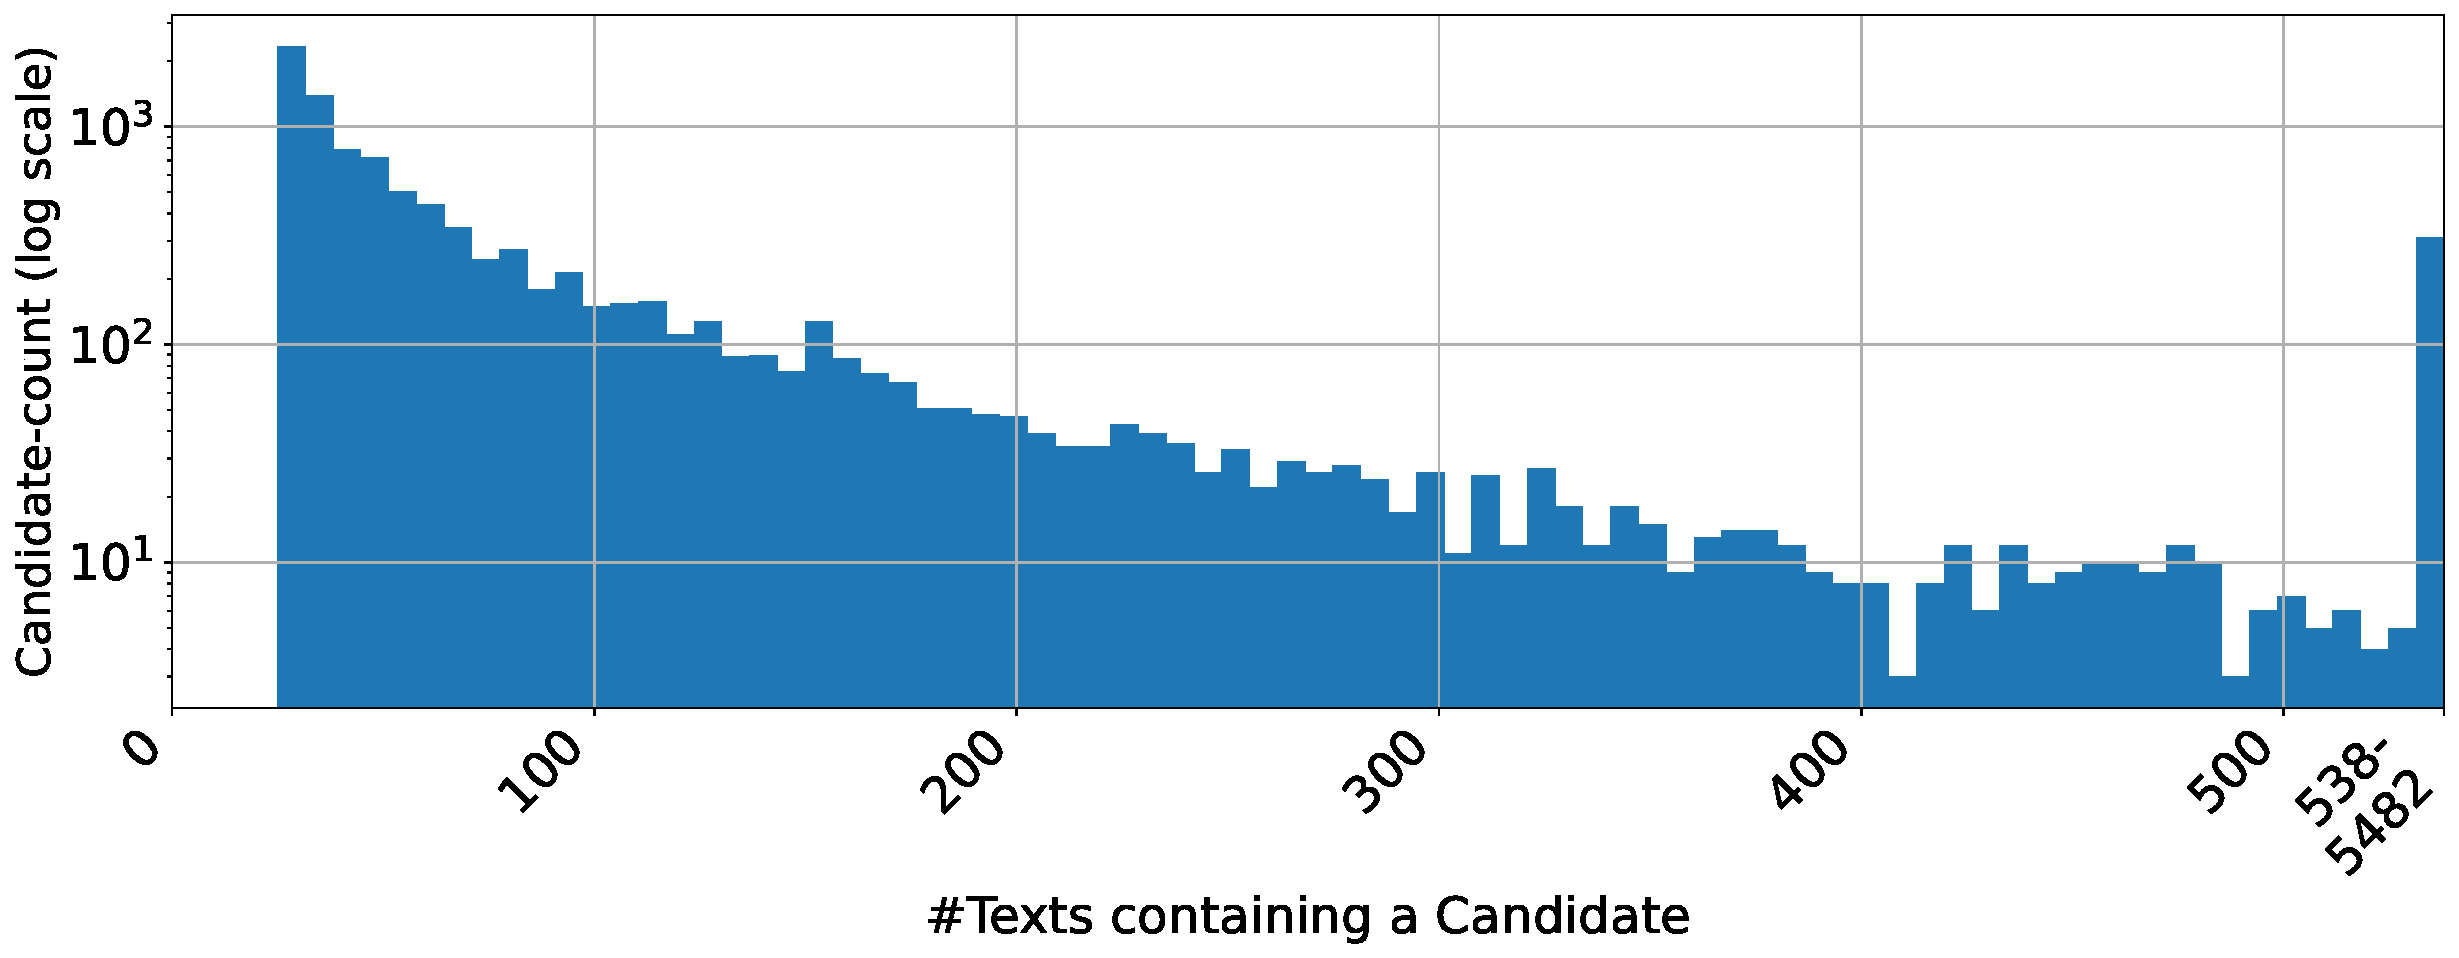
\includegraphics[width=\figwidth]{graphics/dataset_new/docs_per_phrase.pdf}
	\caption[Distribution of texts per candidate]{Distribution of texts per candidate (log scale), cut off at the 97\textsuperscript{th} percentile. \Gls{df}-threshold for a candidate is set to 25, yielding 10\,060 candidates for 11\,601 documents. Median number of documents per candidate is 49 and for the 95\textsuperscript{th} percentile 375. 2595 candidates occur in at least 100 descriptions.}
	% Occurences in all Documents per Keyphrase (for all keyphrases that occur $\geq$ 5 times, cut off at the 93th percentile). 7007 of 45295 terms occur at least 5 times. Most frequent phrases: seminar (4173), course (3722), students (2923), it (2671), language (2071), work (1980), event (1842), research (1731), lecture (1723), law (1719).
	\label{fig:candidate_histogram}
\end{figure}

\todoparagraph{This doesnt look good but lets look at the results!}

\section{Results for the Siddata-dataset}
\label{sec:results_siddata}

As previously described, the primary method used here to check if the described methodology works for the domain of educational resources is to check if low-depth decision trees trained on the extracted semantic directions of the Siddata-dataset can classify a courses' faculty. Before doing that however, it is important to first validate if it can reasonably assumed that the faculty \textit{can generally} be extracted from only the descriptions associated with the entities.





\includeMD{pandoc_generated_latex/4_0_results}

The plots \ref{fig:scatter_mds_movies} and \ref{fig:scatter_mds_placetypes} show a 2D-representation of the MDS %TODO: link MDS anyway, if not to the glossary than to the section
of the movies- and placetypes-dataset as made public by \textcite{Derrac2015}\footnote{\url{https://www.cs.cf.ac.uk/semanticspaces/}}. Visually comparing them to their equivalent to the SIDDATA-dataset (\autoref{fig:scatter_mds}) \todoparagraph{shows that while the movie-embeddings looks pretty clustered}, the clustering of the placetypes-dataset looks in fact a lot worse than that of the SIDDATA-dataset.
%TODO: obviously write again. What do we see? A 2D-Version of the MDS. If we see very distinct clusters in that, we can conclude that it sounds possible that we can detect whatever-we-colored-by from this embeddings to an okay degree.





\section{Qualitative Analysis}

\begin{figure}[h]
	\begin{center}
	  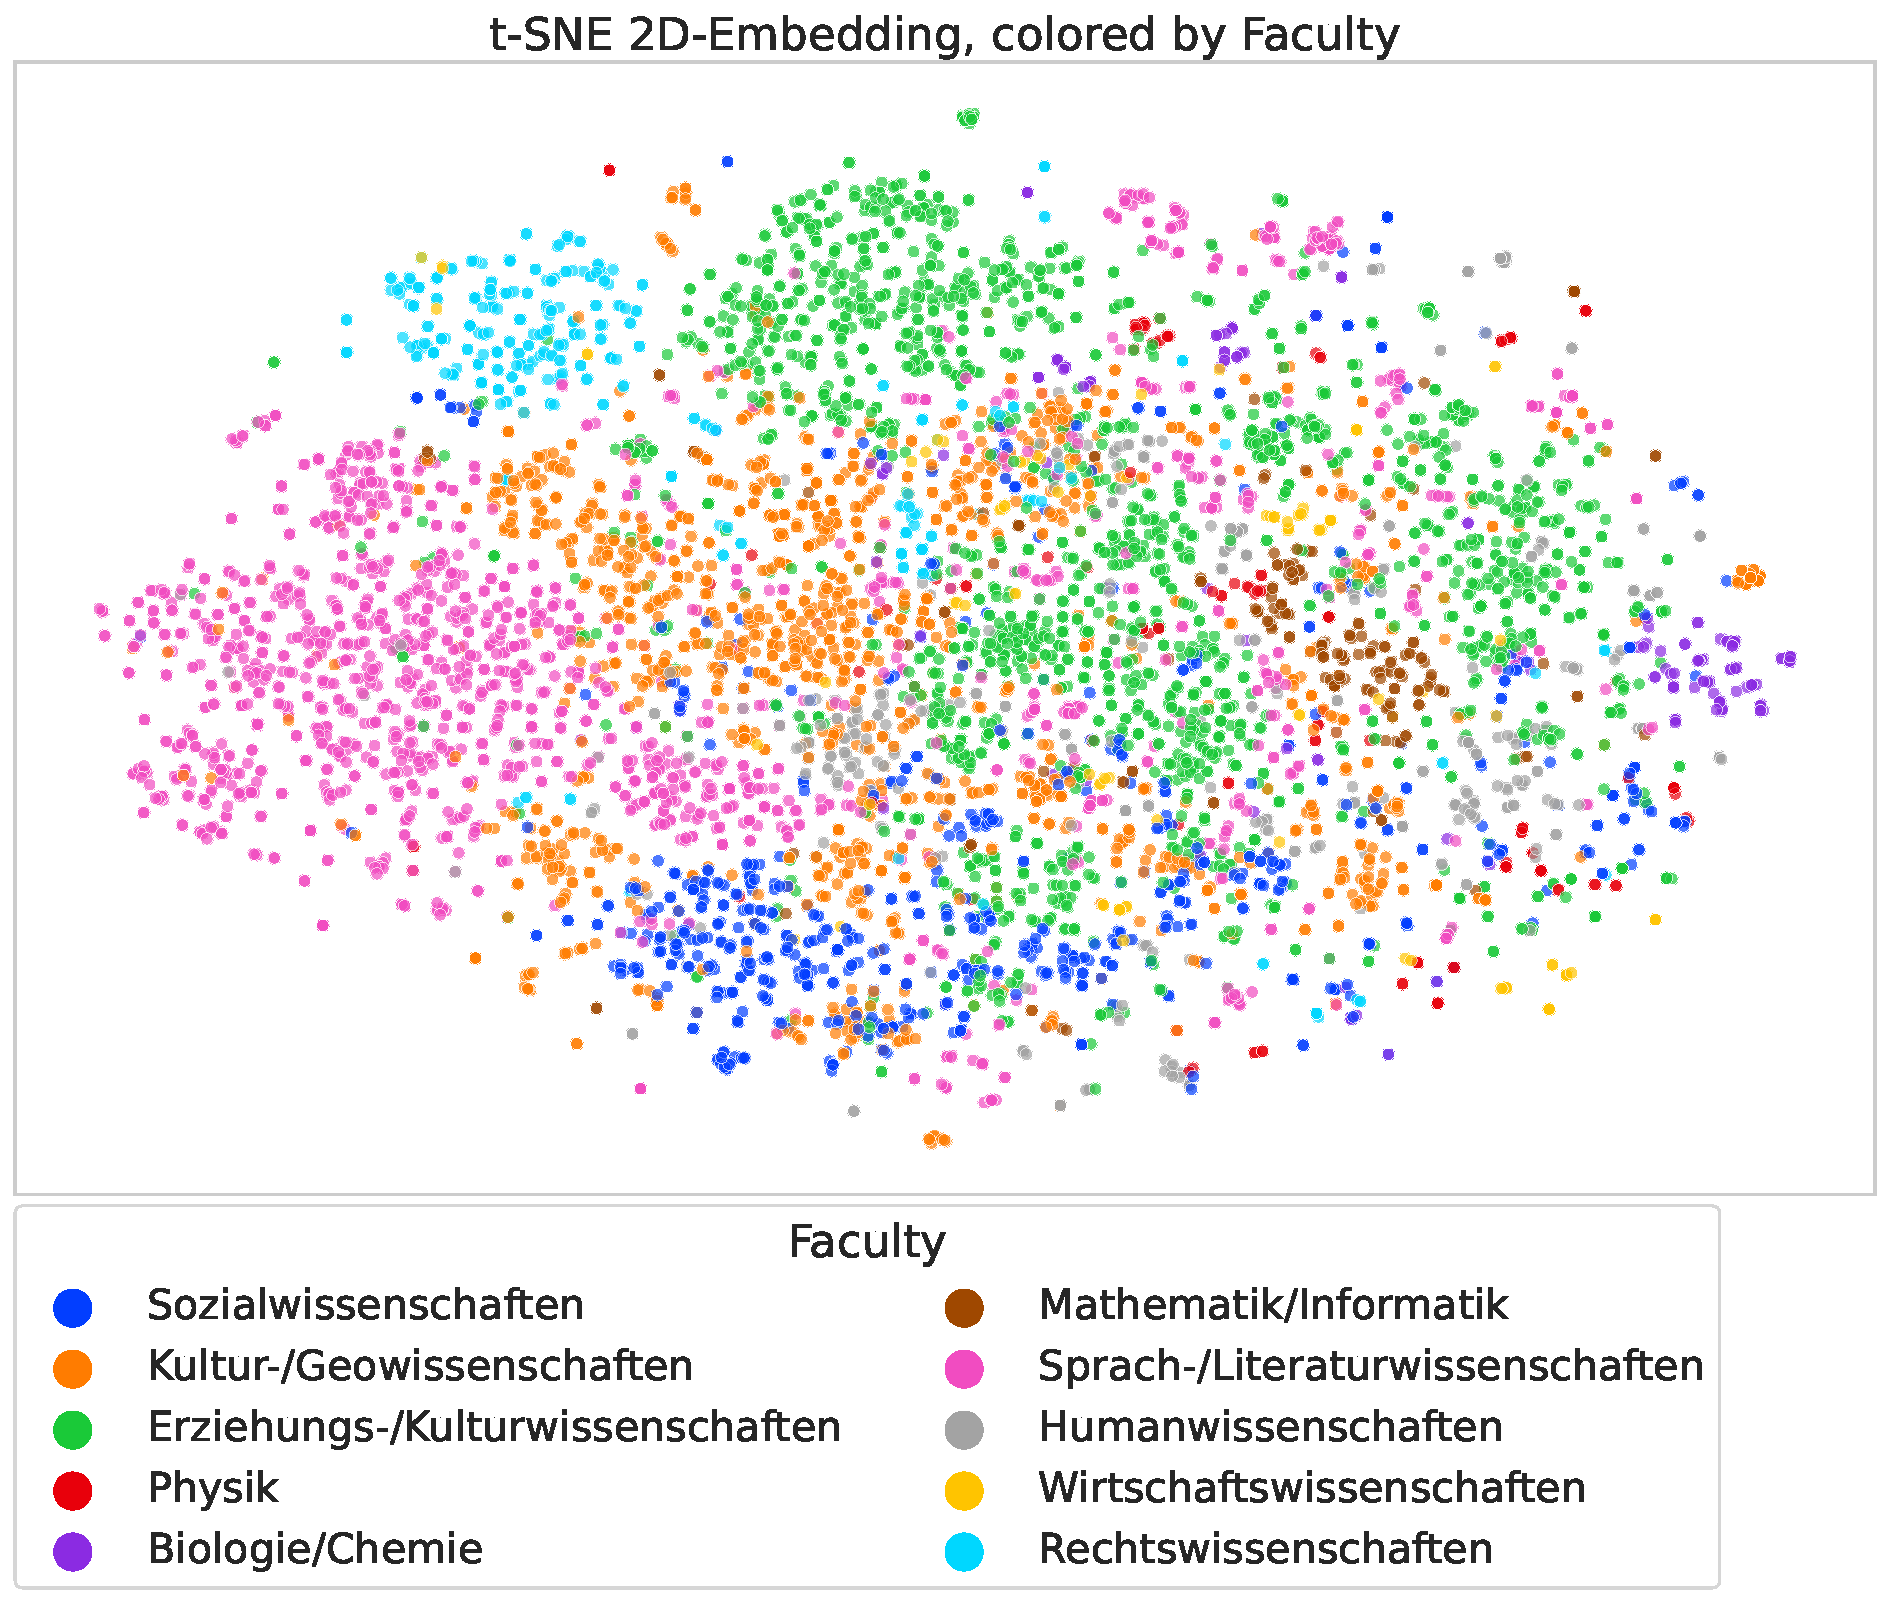
\includegraphics[width=0.9\textwidth]{graphics/dataset_new/scatter_mds_tsne_e2a70a9bf2.pdf}
	  \slcaption{2D Visualization of the Course-Dissimilarity-Matrix, generated with \gls{tsne}. See \url{https://github.com/cstenkamp/derive_conceptualspaces/blob/main/notebooks/text_referenced_plots/visualize_embeddings.ipynb} for the origin of this plot as well as a 3D-plot on unaltered 3D-MDS-data that doesn't rely on t-SNE.}
	  \label{fig:scatter_mds}
	  % möchte sagen: Die Embeddings Clustern -> es lassen sich "sinnvolle Sachen" (wie faculty) draus ziehen.
	\end{center}
\end{figure}



\begin{figure}[h]
	\begin{center}
	  \makebox[\textwidth][c]{
		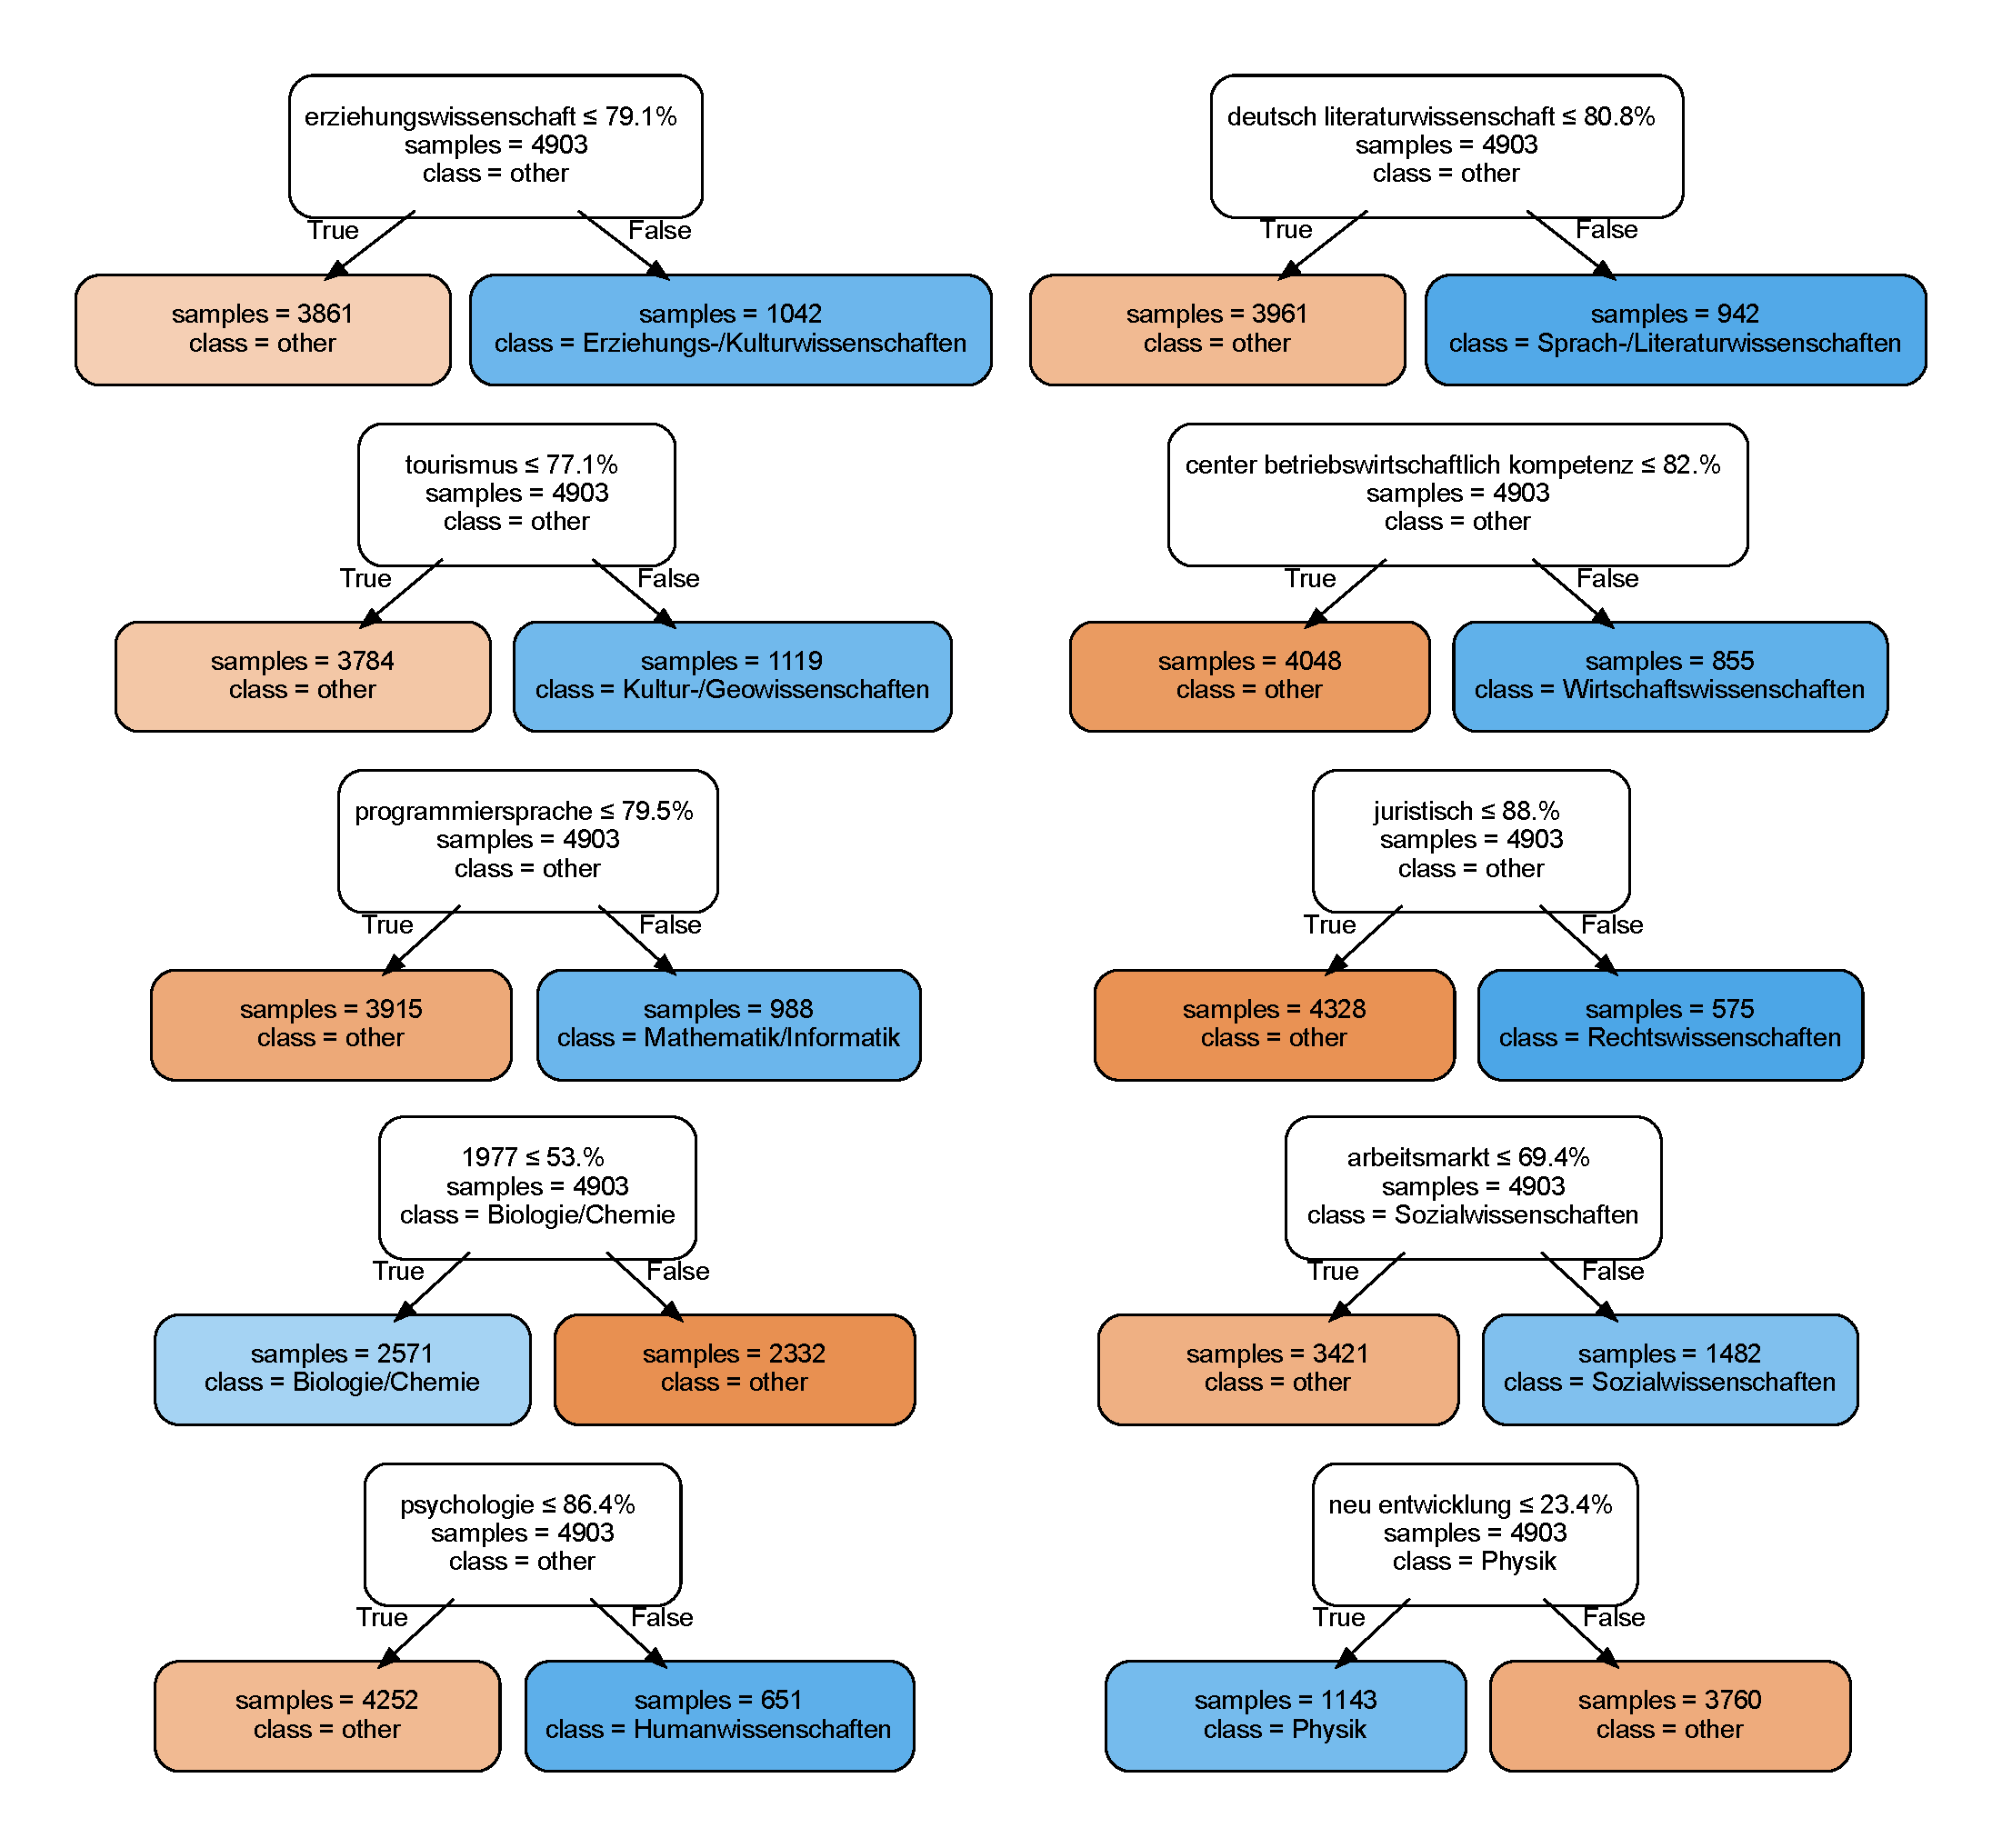
\includegraphics[width=1.3\textwidth]{graphics/dataset_new/dims_for_fb.pdf}
		\slcaption{Learned Level-1-Decisiontrees.}
		\label{fig:dims_for_fb}
		% möchte sagen: Unsere Extracted Dimensions entsprehcen human concepts wie Fachbereich
	  }
	\end{center}
\end{figure}

\begin{figure}[h]
	\begin{center}
	  \makebox[\textwidth][c]{
		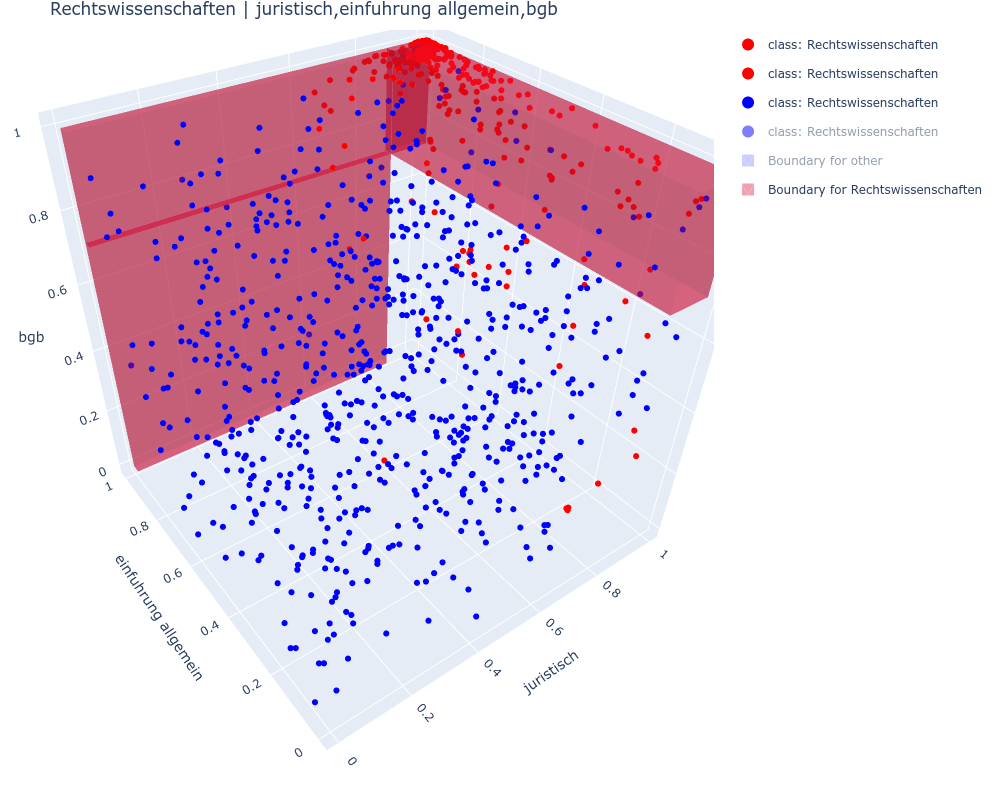
\includegraphics[width=1.1\textwidth]{graphics/dataset_new/boxes_rechtswis.png}
		\slcaption{A classification with a Level-3-Decisiontree. Visualize in 3D: \url{https://github.com/cstenkamp/derive_conceptualspaces/blob/main/notebooks/text_referenced_plots/display_top3_SIDDATA.ipynb} }
		\label{fig:boxes_rechtswis}
		% möchte sagen: How does a decision look graphically, and how does it compare to the original 3D?
		% TODO: add accuracy 
	  }
	\end{center}
\end{figure}


\begin{figure}[h]
	\begin{center}
	  \makebox[\textwidth][c]{
		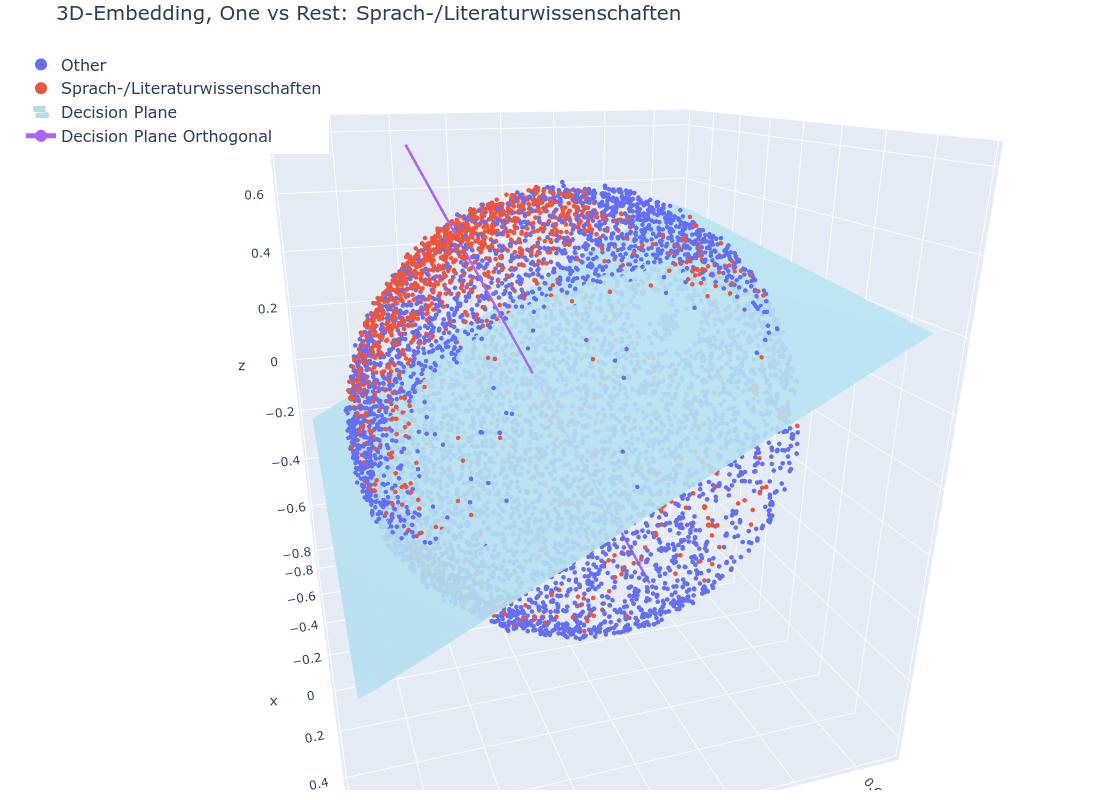
\includegraphics[width=1.1\textwidth]{graphics/dataset_new/possibledecision_sprachlit.png}
		\slcaption{A possible Hyperplane on a 3-Dimensional Embedding. The SVM depicted here would reach an Accuracy of 67.9\% (Precision: 39.8\%, Recall: 70.5\%). Visualize interactively: \url{https://github.com/cstenkamp/derive_conceptualspaces/blob/main/notebooks/text_referenced_plots/visualize_embeddings_mds.ipynb} }
		\label{fig:mds_3d_hyperplane}
		%möchte sagen: To say what the lower boundary of what a 3D-Embedding of NON-CLASS-SPECIFIC dimensions can yield for classification, 
		% wie related der space von fig:boxes_rechtswis mit den interpretable dimensions zu IRGENDEINEM 3D-Space
	  }
	\end{center}
\end{figure}



\begin{figure}[H]
	\centering
	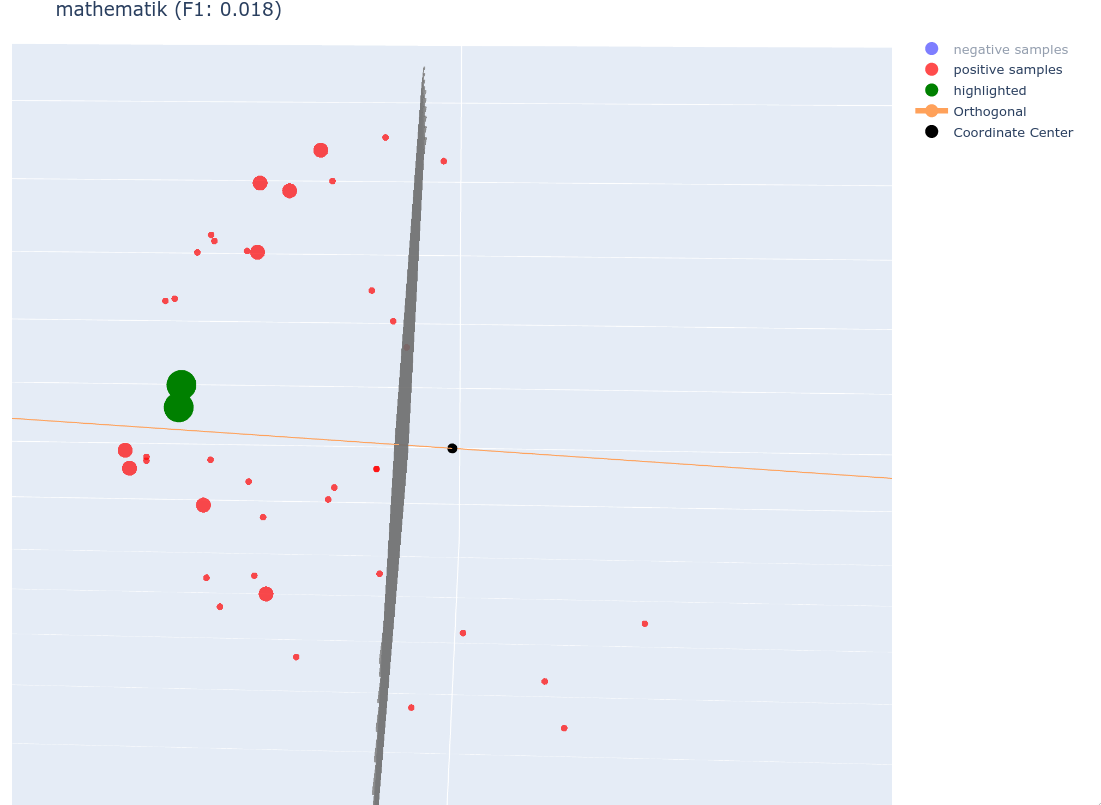
\includegraphics[width=\figwidth]{svm_mathematik_highlight_infoAB.png}
	\caption[3D-Plot with an SVM for the term "Mathematik"]{
		\label{fig:3dplot_mathe_infoab}
		3D-Plot with an SVM for the term "Mathematik", also highlighting the courses "Informatik A" and "Informatik B"
	}
\end{figure}



\section{Quantiative Analysis}

\todoparagraph{As described in} \autoref{sec:workflow}, a good first approximation is to check how many candidate-terms we get. \autoref{tab:kappa_table} shows the results of many runs with different parameter-combinations with the purpose of figuring out which combination of parameters and kappa-metrics lead to enough candidate-terms (\todoparagraph{Also ref the figure of workflow where I check what threshold was realistic})


\begin{table}[h]
	\resizebox{\textwidth}{!}{%
	\begin{tabular}{llllrrrrrrrrr}
	\toprule
% 	 &  &  &  & \rotatebox{70}{\textbf{k_r2r_d}} & \rotatebox{70}{\textbf{k_r2r_min}} & \rotatebox{70}{\textbf{k_dig}} & \rotatebox{70}{\textbf{k_r2r+_d}} & \rotatebox{70}{\textbf{k_r2r+_min}} & \rotatebox{70}{\textbf{k_r2r+_max}} & \rotatebox{70}{\textbf{k_dig+_2}} & \rotatebox{70}{\textbf{k_c2r+}} & \rotatebox{70}{\textbf{mean}} \\
	\textbf{Preprocessing} & \specialcell[b]{\textbf{Quanti-}\\ \textbf{fication}} & \textbf{\#Dims} & \specialcell[b]{\textbf{Doc-Term-}\\ \textbf{Matrix} \\ \textbf{Quanti-}\\ \textbf{fication}} & \rotatebox{70}{\textbf{k_r2r_d}} & \rotatebox{70}{\textbf{k_r2r_min}} & \rotatebox{70}{\textbf{k_dig}} & \rotatebox{70}{\textbf{k_r2r+_d}} & \rotatebox{70}{\textbf{k_r2r+_min}} & \rotatebox{70}{\textbf{k_r2r+_max}} & \rotatebox{70}{\textbf{k_dig+_2}} & \rotatebox{70}{\textbf{k_c2r+}} & \rotatebox{70}{\textbf{mean}} \\
	\midrule
	\multirow[t]{24}{*}{\mfauhcsdT} & \multirow[t]{8}{*}{\textbf{count}} & \multirow[t]{2}{*}{\textbf{3}} & \textbf{ppmi} & 0 & 1 & 0 & 145 & 370 & 510 & 191 & - & 174 \\
	 &  &  & \textbf{tfidf} & 0 & 1 & 0 & 110 & 237 & 278 & 83 & - & 101 \\
	\cline{3-4}
	 &  & \multirow[t]{3}{*}{\textbf{100}} & \textbf{count} & 0 & 5 & 0 & 0 & 114 & 52 & 290 & 0 & 58 \\
	 &  &  & \textbf{ppmi} & 0 & 6 & 27 & 139 & 224 & 247 & 120 & - & 109 \\
	 &  &  & \textbf{tfidf} & 0 & 6 & 5 & 246 & 270 & 281 & 201 & - & 144 \\
	\cline{3-4}
	 &  & \multirow[t]{3}{*}{\textbf{200}} & \textbf{count} & 0 & 5 & 1 & 0 & 133 & 52 & 509 & 0 & 88 \\
	 &  &  & \textbf{ppmi} & 0 & 6 & 57 & 196 & 315 & 344 & 90 & - & 144 \\
	 &  &  & \textbf{tfidf} & 0 & 6 & 17 & 357 & 370 & 372 & 433 & - & 222 \\
	\cline{2-4} \cline{3-4}
	 & \multirow[t]{8}{*}{\textbf{ppmi}} & \multirow[t]{2}{*}{\textbf{3}} & \textbf{ppmi} & 0 & 0 & 0 & 192 & 247 & 363 & 136 & - & 134 \\
	 &  &  & \textbf{tfidf} & 0 & 0 & 0 & 169 & 206 & 217 & 59 & - & 93 \\
	\cline{3-4}
	 &  & \multirow[t]{3}{*}{\textbf{100}} & \textbf{count} & 0 & 0 & 0 & 0 & 38 & 25 & 242 & 0 & 38 \\
	 &  &  & \textbf{ppmi} & 0 & 0 & 0 & 80 & 112 & 101 & 22 & - & 45 \\
	 &  &  & \textbf{tfidf} & 0 & 0 & 0 & 89 & 90 & 96 & 85 & - & 51 \\
	\cline{3-4}
	 &  & \multirow[t]{3}{*}{\textbf{200}} & \textbf{count} & 0 & 0 & 0 & 0 & 34 & 21 & 293 & 0 & 44 \\
	 &  &  & \textbf{ppmi} & 0 & 1 & 112 & 100 & 163 & 163 & 37 & - & 82 \\
	 &  &  & \textbf{tfidf} & 0 & 1 & {\cellcolor{lightgreen}} 127 & 99 & 107 & 106 & 131 & - & 82 \\
	\cline{2-4} \cline{3-4}
	 & \multirow[t]{8}{*}{\textbf{tfidf}} & \multirow[t]{2}{*}{\textbf{3}} & \textbf{ppmi} & 0 & 0 & 0 & 229 & 357 & 423 & 84 & - & 156 \\
	 &  &  & \textbf{tfidf} & 0 & 0 & 0 & 169 & 255 & 258 & 24 & - & 101 \\
	\cline{3-4}
	 &  & \multirow[t]{3}{*}{\textbf{100}} & \textbf{count} & 0 & 1 & 0 & 0 & 162 & 64 & 450 & 0 & 85 \\
	 &  &  & \textbf{ppmi} & 0 & 1 & 3 & 324 & 404 & 423 & 151 & - & 187 \\
	 &  &  & \textbf{tfidf} & 0 & 1 & 0 & 390 & 422 & 437 & 425 & - & 239 \\
	\cline{3-4}
	 &  & \multirow[t]{3}{*}{\textbf{200}} & \textbf{count} & 0 & 2 & 0 & 0 & 211 & 83 & {\cellcolor{lightgreen}} 869 & {\cellcolor{lightgreen}} 1 & 146 \\
	 &  &  & \textbf{ppmi} & 0 & 2 & 13 & 395 & {\cellcolor{lightgreen}} 559 & {\cellcolor{lightgreen}} 577 & 153 & - & 243 \\
	 &  &  & \textbf{tfidf} & 0 & 2 & 0 & {\cellcolor{lightgreen}} 531 & 554 & 572 & 794 & - & {\cellcolor{lightgreen}} 350 \\
	\cline{1-4} \cline{2-4} \cline{3-4}
	\multirow[t]{24}{*}{\mfauhtcsldp} & \multirow[t]{8}{*}{\textbf{count}} & \multirow[t]{2}{*}{\textbf{3}} & \textbf{ppmi} & 0 & 1 & 0 & 226 & 319 & 317 & 208 & - & 153 \\
	 &  &  & \textbf{tfidf} & 0 & 1 & 0 & 210 & 214 & 215 & 82 & - & 103 \\
	\cline{3-4}
	 &  & \multirow[t]{3}{*}{\textbf{100}} & \textbf{count} & 0 & 7 & 0 & 0 & 118 & 61 & 230 & 0 & 52 \\
	 &  &  & \textbf{ppmi} & 0 & 8 & 27 & 184 & 256 & 262 & 125 & - & 123 \\
	 &  &  & \textbf{tfidf} & 0 & 8 & 5 & 253 & 255 & 255 & 168 & - & 135 \\
	\cline{3-4}
	 &  & \multirow[t]{3}{*}{\textbf{200}} & \textbf{count} & 0 & 8 & 0 & 0 & 117 & 64 & 290 & 0 & 60 \\
	 &  &  & \textbf{ppmi} & 0 & {\cellcolor{lightgreen}} 11 & 41 & 200 & 319 & 325 & 88 & - & 141 \\
	 &  &  & \textbf{tfidf} & 0 & {\cellcolor{lightgreen}} 11 & 8 & 331 & 333 & 333 & 302 & - & 188 \\
	\cline{2-4} \cline{3-4}
	 & \multirow[t]{8}{*}{\textbf{ppmi}} & \multirow[t]{2}{*}{\textbf{3}} & \textbf{ppmi} & 0 & 0 & 0 & 138 & 310 & 321 & 254 & - & 146 \\
	 &  &  & \textbf{tfidf} & 0 & 0 & 0 & 143 & 148 & 150 & 187 & - & 90 \\
	\cline{3-4}
	 &  & \multirow[t]{3}{*}{\textbf{100}} & \textbf{count} & 0 & 0 & 0 & 0 & 29 & 11 & 186 & 0 & 28 \\
	 &  &  & \textbf{ppmi} & 0 & 1 & 0 & 117 & 142 & 142 & 20 & - & 60 \\
	 &  &  & \textbf{tfidf} & 0 & 1 & 0 & 122 & 124 & 124 & 103 & - & 68 \\
	\cline{3-4}
	 &  & \multirow[t]{3}{*}{\textbf{200}} & \textbf{count} & 0 & 1 & 0 & 0 & 25 & 10 & 272 & 0 & 38 \\
	 &  &  & \textbf{ppmi} & 0 & 1 & 48 & 126 & 161 & 165 & 28 & - & 76 \\
	 &  &  & \textbf{tfidf} & 0 & 1 & 17 & 143 & 144 & 148 & 133 & - & 84 \\
	\cline{2-4} \cline{3-4}
	 & \multirow[t]{8}{*}{\textbf{tfidf}} & \multirow[t]{2}{*}{\textbf{3}} & \textbf{ppmi} & 0 & 0 & 0 & 146 & 219 & 223 & 133 & - & 103 \\
	 &  &  & \textbf{tfidf} & 0 & 0 & 0 & 108 & 111 & 109 & 38 & - & 52 \\
	\cline{3-4}
	 &  & \multirow[t]{3}{*}{\textbf{100}} & \textbf{count} & 0 & 1 & 0 & 0 & 160 & 54 & 389 & 0 & 76 \\
	 &  &  & \textbf{ppmi} & 0 & 2 & 9 & 281 & 375 & 380 & 205 & - & 179 \\
	 &  &  & \textbf{tfidf} & 0 & 2 & 0 & 373 & 377 & 392 & 339 & - & 212 \\
	\cline{3-4}
	 &  & \multirow[t]{3}{*}{\textbf{200}} & \textbf{count} & 0 & 3 & 0 & 0 & 199 & 64 & 661 & 0 & 116 \\
	 &  &  & \textbf{ppmi} & 0 & 3 & 21 & 362 & 456 & 472 & 164 & - & 211 \\
	 &  &  & \textbf{tfidf} & 0 & 3 & 1 & 499 & 498 & 501 & 645 & - & 307 \\
	\bottomrule
	\end{tabular}
	}
	\caption{Number of Candidate-Phrases for different parameter-combinations and kappa-values \label{tab:kappa_table}}
	\label{tab:cands_per_config}
\end{table}



\begin{table}
	\caption{Duplicates per Combination of n-dims and n-categories-per-dim}
	\begin{tabular}{lrrrrrr}
	\toprule
	 & \textbf{2} & \textbf{11} & \textbf{23} & \textbf{116} & \textbf{232} & \textbf{1160} \\
	\#dims &  &  &  &  &  &  \\
	\midrule
	3 & 100\% & 99.85\% & 68.98\% & 6.85\% & 5.25\% & 3.97\% \\
	5 & 100\% & 24.91\% & 9.79\% & 5.25\% & 4.72\% & 3.42\% \\
	10 & 100\% & 10.18\% & 6.90\% & 4.67\% & 4.23\% & 2.11\% \\
	20 & 100\% & 7.41\% & 5.58\% & 4.23\% & 3.52\% & 0.79\% \\
	50 & 99.97\% & 5.46\% & 4.72\% & 3.19\% & 1.89\% & 0.05\% \\
	100 & 99.88\% & 4.80\% & 4.18\% & 1.94\% & 0.65\% & 0\% \\
	200 & 99.55\% & 4.36\% & 3.44\% & 0.67\% & 0.09\% & 0\% \\
	\bottomrule
	\end{tabular}
\end{table}


\begin{table}
	\resizebox{\textwidth}{!}{%
	\begin{tabular}{rlllcc}
	& & & & \multicolumn{2}{c}{\textbf{Prediction Accuracy}} \\
	\textbf{Faculty} & \multicolumn{3}{c}{\textbf{Top 3 Directions}} & \textbf{Depth 3} & \textbf{Depth 1} \\
	\midrule
	\textbf{Erziehungs-/Kulturwissenschaften} & erziehungswissenschaft & okumenisch & english for & 78.02\% & 75.50\% \\
	\textbf{Rechtswissenschaften} & juristisch & bgb & bgb & 95.86\% & 91.10\% \\
	\textbf{Wirtschaftswissenschaften} & {\scriptsize center betriebswirtschaftlich kompetenz } & religionsunterrichts & design & 89.65\% & 79.10\% \\
	\textbf{Kultur-/Geowissenschaften} & tourismus & gi & stadtgeographie & 75.50\% & 77.44\% \\
	\textbf{Mathematik/Informatik} & programmiersprache & menge & hoffnung & 93.00\% & 91.85\% \\
	\textbf{Sprach-/Literaturwissenschaften} & deutsch literaturwissenschaft & sprache & okumenisch & 86.71\% & 85.10\% \\
	\textbf{Humanwissenschaften} & psychologie & metaphysik & internationalisierung & 86.84\% & 85.51\% \\
	\textbf{Physik} & neu entwicklung & mitarbeiterinnen & {\small regelmassig aktiv teilnahme} & 78.27\% & 77.36\% \\
	\textbf{Biologie/Chemie} & aktivierung studierend & brd & berucksichtigung finden & 85.22\% & 62.13\% \\
	\textbf{Sozialwissenschaften} & arbeitsmarkt & regieren & multiple & 78.60\% & 67.63\% \\
	\end{tabular}
	\caption{Top 3 Directions to detect the respective faculty from the data. a (!) behind a direction means that its inversed (LOW values point towards the class)}
	\label{tab:courses_top3}
	}
\end{table}


% Please add the following required packages to your document preamble:
% \usepackage{graphicx}
\begin{table}[]
	\centering
	\resizebox{\textwidth}{!}{%
	\begin{tabular}{rlllcc}
	\multicolumn{1}{l}{} &                                               &  &  & \multicolumn{2}{c}{\textbf{Prediction Accuracy}} \\
	\textbf{Faculty}     & \multicolumn{1}{c}{\textbf{Top 3 Directions}} &  &  & \textbf{Top 1}          & \textbf{Top 3}         \\
	\textbf{Erziehungs-/Kulturwissenschaften} & padagogisch    &  &  &  &  \\
	\textbf{Rechtswissenschaften}             & recht          &  &  &  &  \\
	\textbf{Wirtschaftswissenschaften}        & management     &  &  &  &  \\
	\textbf{Kultur-/Geowissenschaften}        & geographisch   &  &  &  &  \\
	\textbf{Mathematik/Informatik}            & computer       &  &  &  &  \\
	\textbf{Sprach-/Literaturwissenschaften}  & literarisch    &  &  &  &  \\
	\textbf{Humanwissenschaften}              & therapeutisch  &  &  &  &  \\
	\textbf{Physik}                           & gestik         &  &  &  &  \\
	\textbf{Biologie/Chemie}                  & geschichte (!) &  &  &  &  \\
	\textbf{Sozialwissenschaften}             & politik        &  &  &  & 
	\end{tabular}%
	}
	\caption{Top 3 Directions to detect the respective faculty from the data. a (!) behind a direction means that its inversed (LOW values point towards the class)}
	\label{tab:courses_top3_2}
\end{table}



% Other configs: {'dataset': 'siddata2022', 'debug': 'False', 'prim_lambda': '0.5', 'sec_lambda': '0.2', 'classifier_succmetric': 'kappa_digitized_onlypos_2', 'cluster_direction_algo': 'reclassify', 'kappa_weights': 'quadratic', 'embed_dimensions': '200', 'embed_algo': 'mds', 'quantification_measure': 'tfidf', 'dcm_quant_measure': 'count', 'extraction_method': 'tfidf', 'translate_policy': 'onlyorig', 'pp_components': 'mfauhtcsldp', 'language': 'de', 'min_words_per_desc': '80'}
% Args for best Tree: balance_classes=True, one_vs_rest=True, dt_depth=1, test_percentage_crossval=0.33
\begin{table}
	\resizebox{\textwidth}{!}{%
	\caption{Decision-Tree-Accuracies for different Parameter-Combinations}
	\begin{tabular}{lllrrrrrr}
	\toprule
	 &  &  & \textbf{ppmi} & \textbf{ppmi} & \textbf{ppmi} & \textbf{tfidf} & \textbf{tfidf} & \textbf{tfidf} \\
	pp_components & dcm_quant_measure & classifier_succmetric &  &  &  &  &  &  \\
	\midrule
	\multirow[t]{7}{*}{mfauhcsd2} & \multirow[t]{3}{*}{count} & k_c2r+ & - & 40.58\% & 38.76\% & 36.24\% & 45.16\% & - \\
	 &  & k_dig+_2 & - & 74.83\% & 77.10\% & 74.82\% & 80.42\% & - \\
	 &  & k_r2r+_min & - & 73.59\% & 74.91\% & 77.58\% & 80.71\% & - \\
	\cline{2-3}
	 & \multirow[t]{2}{*}{ppmi} & k_dig+_2 & 62.11\% & 58.63\% & 61.94\% & 79.97\% & - & - \\
	 &  & k_r2r+_min & {\cellcolor{lightgreen}} 70.75\% & 75.52\% & 74.12\% & 81.10\% & - & - \\
	\cline{2-3}
	 & \multirow[t]{2}{*}{tfidf} & k_dig+_2 & 57.86\% & 76.35\% & 76.88\% & 77.58\% & 80.49\% & - \\
	 &  & k_r2r+_min & 67.31\% & 73.45\% & 72.65\% & 77.17\% & 78.81\% & - \\
	\cline{1-3} \cline{2-3}
	\multirow[t]{7}{*}{mfauhtcsldp} & \multirow[t]{3}{*}{count} & k_c2r+ & 49.72\% & 40.70\% & 41.94\% & 53.79\% & 49.17\% & 63.38\% \\
	 &  & k_dig+_2 & 58.25\% & 74.86\% & 77.67\% & 78.00\% & 79.73\% & 44.39\% \\
	 &  & k_r2r+_min & 66.51\% & 72.03\% & 69.78\% & 78.45\% & 79.15\% & 61.95\% \\
	\cline{2-3}
	 & \multirow[t]{2}{*}{ppmi} & k_dig+_2 & - & - & 65.67\% & 77.58\% & 80.08\% & 58.58\% \\
	 &  & k_r2r+_min & - & - & {\cellcolor{lightgreen}} 80.41\% & {\cellcolor{lightgreen}} 81.41\% & {\cellcolor{lightgreen}} 81.41\% & {\cellcolor{lightgreen}} 64.36\% \\
	\cline{2-3}
	 & \multirow[t]{2}{*}{tfidf} & k_dig+_2 & 64.88\% & 76.31\% & 77.81\% & 77.24\% & - & 59.18\% \\
	 &  & k_r2r+_min & 58.92\% & {\cellcolor{lightgreen}} 78.05\% & 76.49\% & 77.09\% & - & 63.02\% \\
	\bottomrule
	\end{tabular}
	}
\end{table}



\begin{table}[]
	\centering
	\begin{tabular}{r|ll}
	\textbf{Dimension}               & \textbf{reclassify} & \textbf{main}       \\ \midrule
	\textbf{isawyoufirst}            & beach               & beach               \\
	\textbf{workspace}               & office              &                     \\
	\textbf{nutrition}               & restaurant          & deli                \\
	\textbf{goalie}                  & stadium             & footballstadium     \\
	\textbf{pumperbuilding}          & county              &                     \\
	\textbf{starwoodhotels}          & hotelroom           & pool                \\
	\textbf{interstate10}            & highway             & mongolianrestaurant \\
	\textbf{urban}                   & interior            & movietheater        \\
	\textbf{tuolumne}                & creek               & nationalforest      \\
	\textbf{cabs}                    & downtown            &                     \\
	\textbf{investment}              & school              & stockexchange       \\
	\textbf{stripmall}               & downtown            & departmentstore     \\
	\textbf{michiganstateuniversity} & school              & campus              \\
	\textbf{ews}                     & railroad            & train               \\
	\textbf{anchored}                & boat                & pier                \\
	\textbf{a10}                     & airport             &                     \\
	\textbf{wc2}                     & restaurant          & square              \\
	\textbf{airbase}                 & airport             & airbase             \\
	\textbf{joshuatreenationalpark}  & canyon              &                     \\
	\textbf{clinker}                 & building            &                    
	\end{tabular}
	\caption{Highest-ranking descriptions per dimension for the reclassify-algorithm and the main-algorithm}
	\label{tab:text_per_dim}
\end{table}

